\documentclass{article}

\usepackage{graphicx}
\usepackage{tikz}
\usepackage{tikzsymbols}
\usetikzlibrary{calc,patterns,shapes.geometric}
\pagestyle{empty}
\usepackage[margin=0pt]{geometry}
\geometry{papersize={14in,12in}}

\def\centerarc[#1](#2)(#3:#4:#5){\draw[#1] ($(#2)+({#5*cos(#3)},{#5*sin(#3)})$) arc (#3:#4:#5);}

\begin{document}
	\begin{figure}
		\centering
		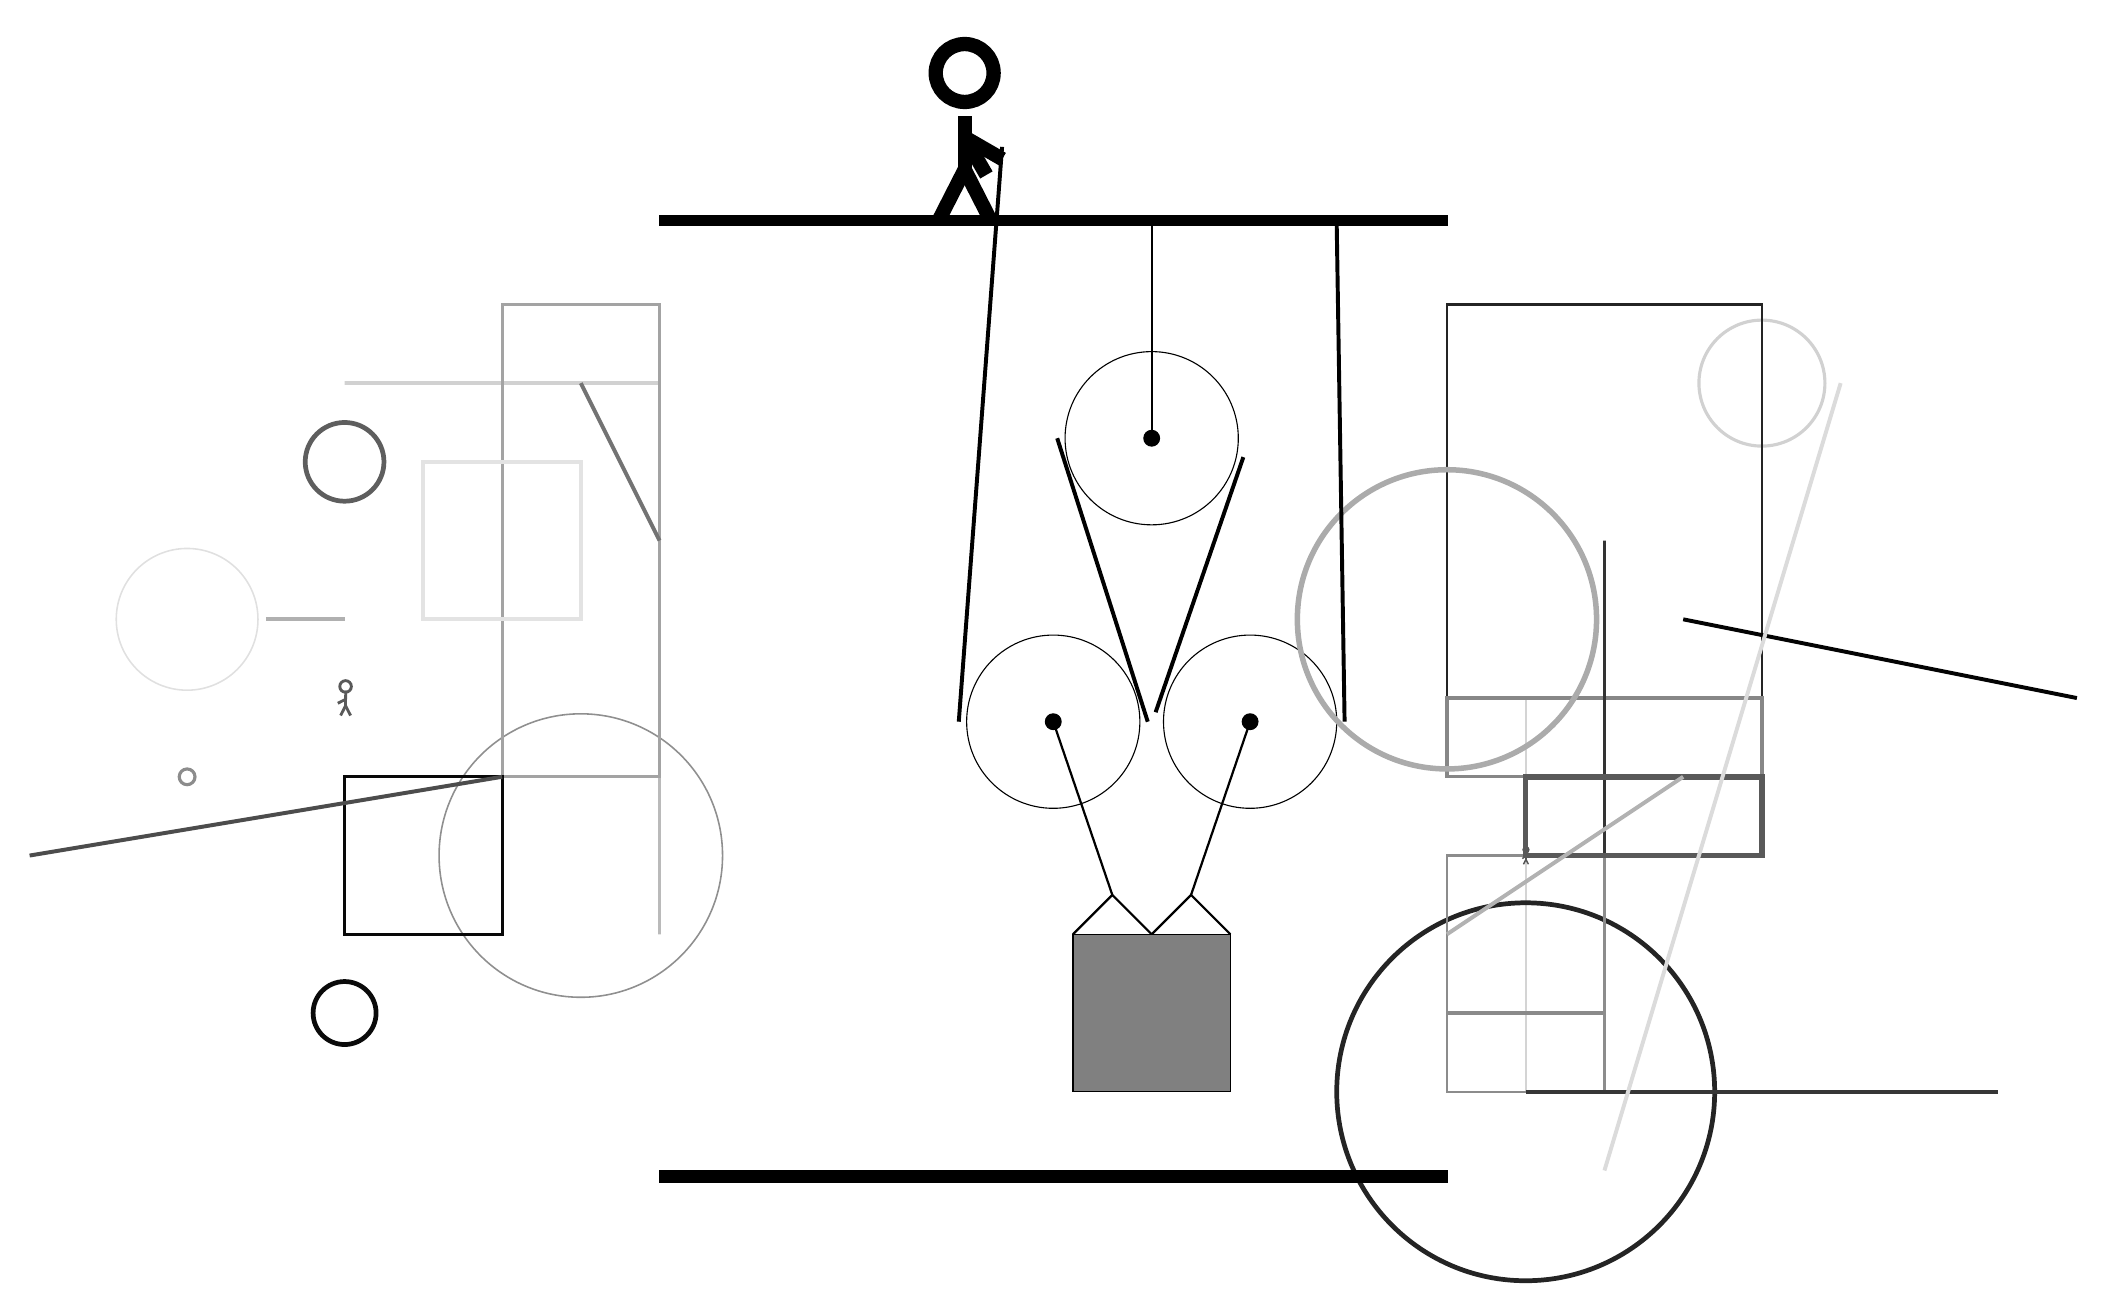
\begin{tikzpicture}
			%%%%% START %%%%%
			
			\draw[fill=black] (-4, 9) rectangle (6, 9.125);
			
			\draw (1, 2.7) circle (1.1);
			\draw[fill=black] (1, 2.7) circle (0.1);
			
			\draw (2.25, 6.3) circle (1.1);
			\draw[fill=black] (2.25, 6.3) circle (0.1);
			\draw[thick] (2.25, 6.3) -- (2.25, 9);
			
			\draw (3.5, 2.7) circle (1.1);
			\draw[fill=black] (3.5, 2.7) circle (0.1);
			
			\draw[thick] (3.5, 2.7) -- (2.75, 0.5);
			\draw[thick] (1, 2.7) -- (1.75, 0.5);
			\draw[thick]  (1.25, 0) -- (1.75, 0.5) -- (2.25, 0);
			\draw[thick]  (2.25, 0) -- (2.75, 0.5) -- (3.25, 0);
			\draw[fill=black!50] (1.25, 0) rectangle (3.25, -2);
			
			\draw[line width=0.3mm, color=black!27] (-4, 0) rectangle (-4, 2);
			
			\draw [line width=0.4mm, color=black!18](10, 7) circle (0.8);
			\draw [line width=0.2mm, color=black!44](-5, 1) circle (1.8);
			\draw[line width=0.2mm, color=black!17] (7, -2) rectangle (8, 3);
			
			\draw[line width=0.3mm, color=black!86] (6, 8) rectangle (10, 2);
			\draw[line width=0.5mm, color=black!18] (-4, 7) rectangle (-8, 7);
			\draw [line width=0.6mm, color=black!86](7, -2) circle (2.4);
			
			\draw[line width=0.5mm, color=black!46] (6, -1) rectangle (8, -1);
			\draw [line width=0.4mm, color=black!45](-10, 2) circle (0.1);
			\draw[line width=0.4mm, color=black!36] (-4, 8) rectangle (-6, 2);
			\node[line width=0.3mm, color=black!65] at (-8, 3) {\Strichmaxerl[2][27][88]};
			\draw [line width=0.6mm, color=black!63](-8, 6) circle (0.5);
			\draw[line width=0.4mm, color=black!47] (6, 2) rectangle (10, 3);
			
			\draw [line width=0.7mm, color=black!33](6, 4) circle (1.9);
			\draw[line width=0.4mm, color=black!80] (8, 0) rectangle (8, 5);
			\node[line width=0.4mm, color=black!68] at (7, 1) {\Strichmaxerl[1][33][44]};
			
			\draw[line width=0.4mm, color=black!97] (-6, 0) rectangle (-8, 2);
			
			\draw[line width=0.3mm, color=black!45] (8, -2) rectangle (6, 1);
			\draw[line width=0.5mm, color=black!99](9, 4) -- (14, 3);
			\draw[line width=0.5mm, color=black!55](-5, 7) -- (-4, 5);
			\draw[line width=0.5mm, color=black!79](7, -2) -- (13, -2);
			\draw[line width=0.7mm, color=black!65] (7, 2) rectangle (10, 1);
			
			\draw[line width=0.5mm, color=black!11] (-5, 4) rectangle (-7, 6);
			\draw[line width=0.5mm, color=black!70](-6, 2) -- (-12, 1);
			\draw [line width=0.2mm, color=black!12](-10, 4) circle (0.9);
			\draw[line width=0.5mm, color=black!30](6, 0) -- (9, 2);
			\draw[line width=0.5mm, color=black!14](8, -3) -- (11, 7);
			\draw[line width=0.5mm, color=black!31](-9, 4) -- (-8, 4);
			\draw [line width=0.6mm, color=black!96](-8, -1) circle (0.4);
			
			\draw[line width=0.5mm] (0.35, 10) --  (-0.2, 2.7);
			\centerarc[line width=0.5mm](1, 2.7)(180:360:1.2000000000000002);
			\draw[line width=0.5mm] (2.2, 2.7) -- (1.05, 6.3);
			\centerarc[line width=0.5mm](2.25, 6.3)(-20:180:1.2000000000000002);
			\draw[line width=0.5mm](3.414, 6.06) -- (2.3, 2.82);
			\centerarc[line width=0.5mm](3.5, 2.7)(160:360:1.2000000000000002);
			\draw[line width=0.5mm](4.7, 2.7) -- (4.6, 9);
			
			\node at (-0.07, 10.2) {\Strichmaxerl[10][120][-30]};
			
			\draw[fill=black] (-4, -3) rectangle (6, -3.15);
			
			%%%%% END %%%%%
		\end{tikzpicture}
	\end{figure}	
\end{document}